\ppageno=15
\ppreviouspageno=14
\plineno=39
\psublineno=1

\newParkoszpage

{\relsize{-1}
\url{http://wbl.klf.uw.edu.pl/13/2/iParkosz.djvu?djvuopts=&page=55&zoom=width&showposition=0.5,0.18}

\url{http://wbl.klf.uw.edu.pl/13/2/iParkosz.djvu?djvuopts=&page=78&zoom=width&showposition=0.5,0.81}
}

\bigskip

\obeylines
\mono



\fullpreviouslines


{
\color{blue}

Tamen 

eciam in suis locis possemus singulas predictas 
}

\plineno=0

\fulllines

litteras seu earum exempla ponere, sicut et ponemus. Non

est enim vicium idem pluries repetere ex causa notandum.

% \def\splitlines{\advance\plineno by 1\psublineno=0\everypar{\advance\psublineno by 1\llap{\textcolor{green}{\the\ppageno-\ifnum\plineno<10 0\fi\the \plineno-\the\psublineno \ }}}}

% \def\newsplitline{\advance\plineno by 1}

\def\splitverse{\advance\plineno by 1\psublineno=0\everypar{\advance\psublineno by 1\llap{\textcolor{green}{\the\ppageno-\ifnum\plineno<10 0\fi\the \plineno-\the\psublineno \ }}\hskip5em}}

% nie działa licznik wierszy?
\def\fullverselines{\everypar{\advance\plineno by 1\llap{\the\ppageno-\ifnum\plineno<10 0\fi\the \plineno \hskip 1.5em}\hskip5em}}


\def\newverse{\advance\plineno by 1\psublineno=0\hskip10em}
\def\newversesubline{\hskip10em}
\def\newverseline{\advance\plineno by 1\psublineno=0}
\def\indentVerse{\hskip10em}

% MUFI SHORT VIRGULA

{

\catcode`\/=13
\def/{{\fontCardo }}



% 
\includegraphics[width=\hsize]{wierszP1m}

\splitverse

Ktho chce piſſaç doſkoɲaɬe

\indentVerse Ġøzik poɬſki

% 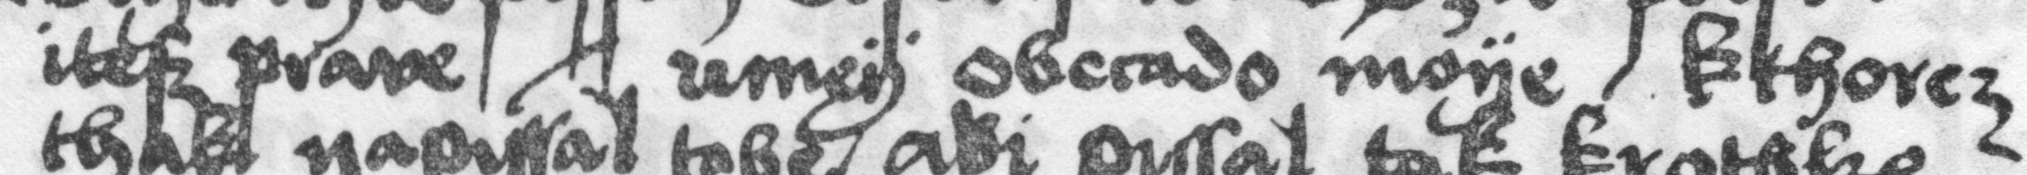
\includegraphics[width=\hsize]{wierszP2}

%\newverse 
\splitverse

itefz prave/


\indentVerse uṁeij obecado ṁoije/

% http://en.wikipedia.org/wiki/Ezh
% 'LATIN SMALL LETTER EZH' (U+0292)
	

\catcode `\^^M=5
\newtip{85}{Tak w rkp., z pewnością należy czytać \textit{ktorem}, a nie \textit{któreż}, co jednak
nie jest o tyle pewne, że w wyrazach, polskich w traktacie skrótów nie ma.}
\obeylines
kthore\conf{ʒ}{}¹

% 85 Tak w rkp., z pewnością należy czytać Morem, a nie któreś, Co jednak

% nie jest o tyle pewne, że w wyrazach, polskich w traktacie skrótów nie ma.

% 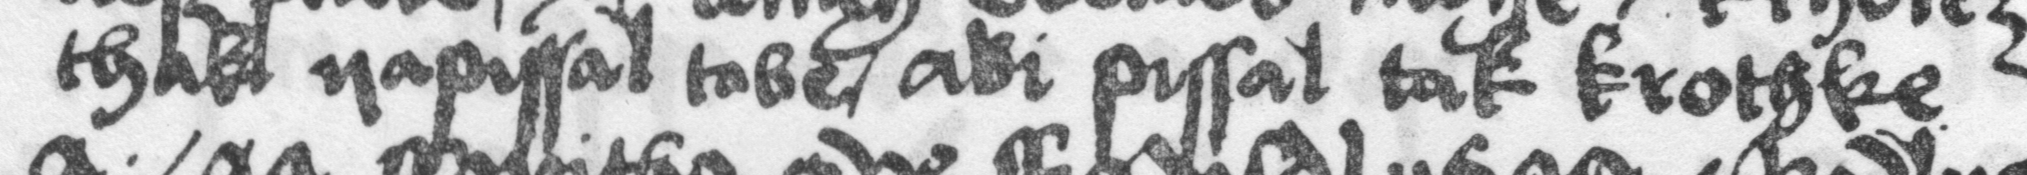
\includegraphics[width=\hsize]{wierszP3}


\splitverse

thak ɲapiſſaḷ toɓe/	

\indentVerse  aɓi piſſaḷ tak krothke 

% 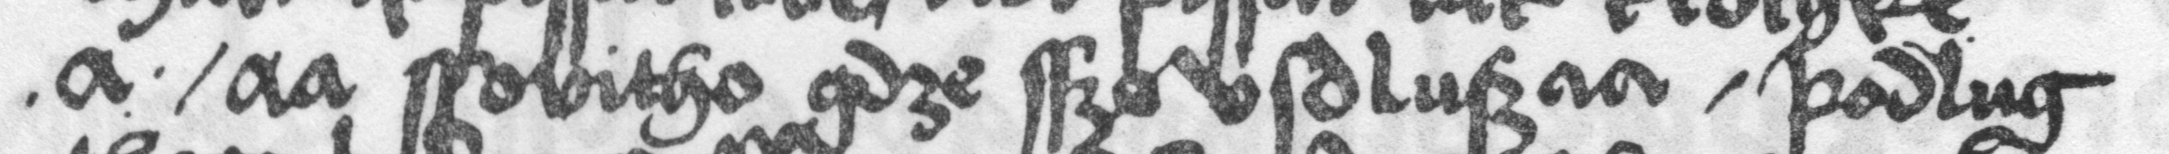
\includegraphics[width=\hsize]{wierszP4}

\splitverse

• a •/

\indentVerse  \textit{aa} ſſovitho ꝿdze ſſzø ʋſdḷuſzaa/

\indentVerse  podḷuꝿ 

% 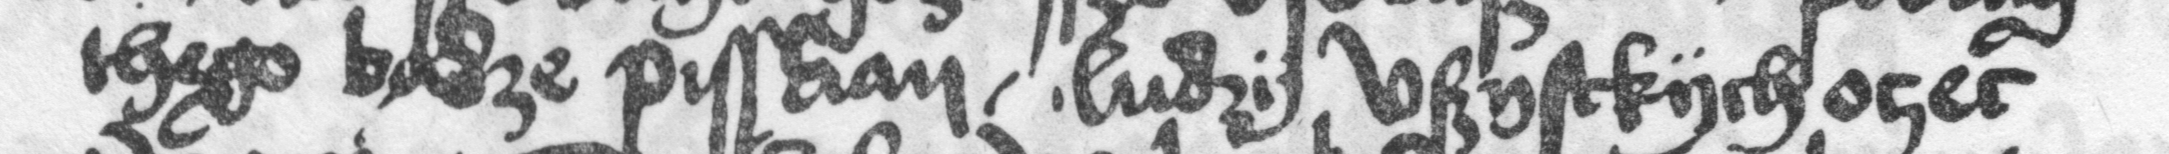
\includegraphics[width=\hsize]{wierszP5}

\splitverse

theꝿo bødze piſſaaɲ/

% znika e!!!
\indentVerse ɬudzij ʋſzyſtkijch oçec 

\newpage
% 
\includegraphics[width=\hsize]{wierszP6}

\splitverse

\textit{adaaɱ}/

\indentVerse A theſz ġdze • ƀ • bødze ġruube/ 

% \newverseline

% 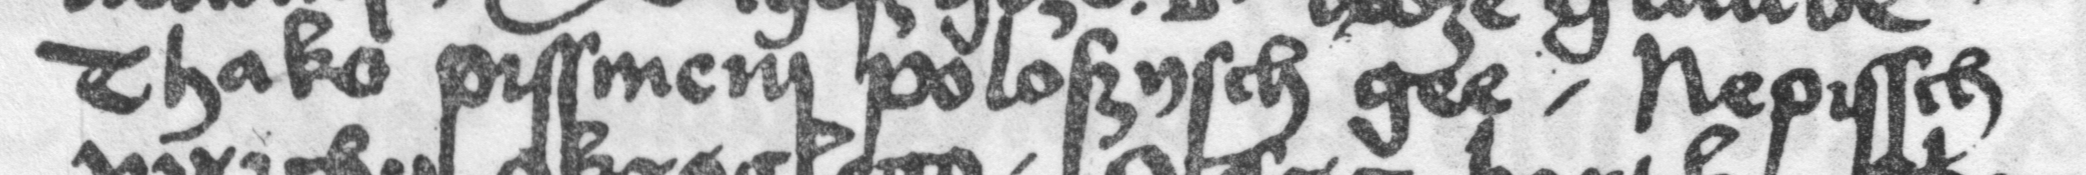
\includegraphics[width=\hsize]{wierszP7}

\splitverse

Thako piſſṁeɱ poḷoſzyſch ġee/

\newversesubline Ṅepiſſch 

% 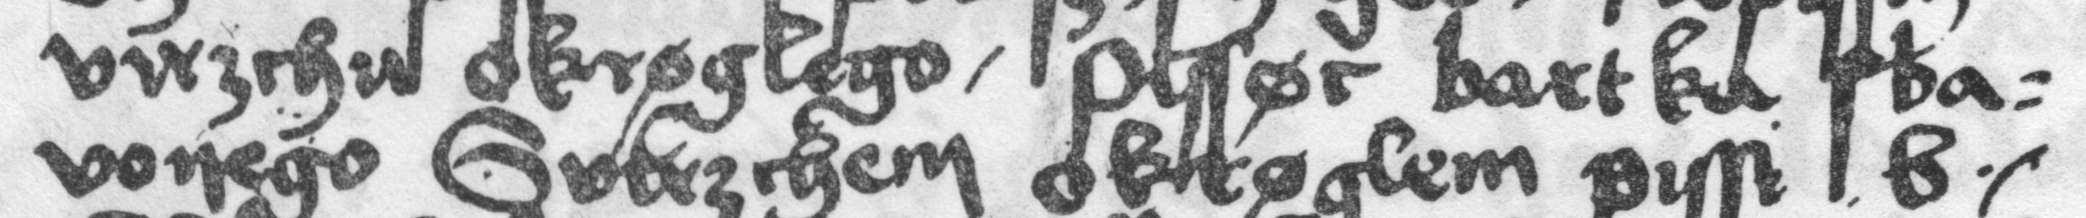
\includegraphics[width=\hsize]{wierszP8}

\splitverse virzchu okrøꝿɬeꝿo/

% hyphen!!!
\newversesubline Piſſøc \textit{bartka} \textit{\hyphh{ſba}{voɲeġo}}

% 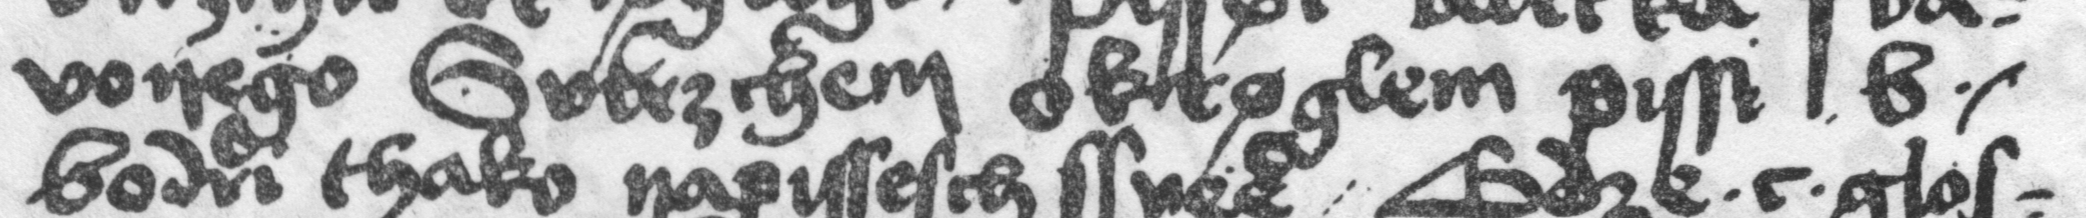
\includegraphics[width=\hsize]{wierszP9}

%\newverseline
\fullverselines

 \textit{\hypht{ſba}{voɲeġo}} Svirzcheɱ okrøꝿɬeṁ piſſi • ɓ •/

% 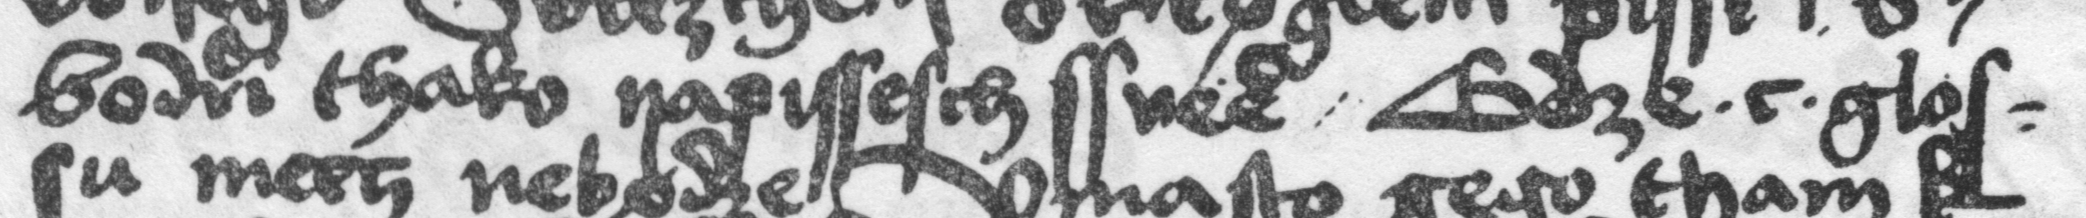
\includegraphics[width=\hsize]{wierszP10}

\plineno=12
\splitverse

\textit{ɓodri} thako ɲapiſſeſch ſſvee/

% zły numer!

\indentVerse Ġdze • \textit{c} • \hyphh{ġḷoſ}{ſu}

% 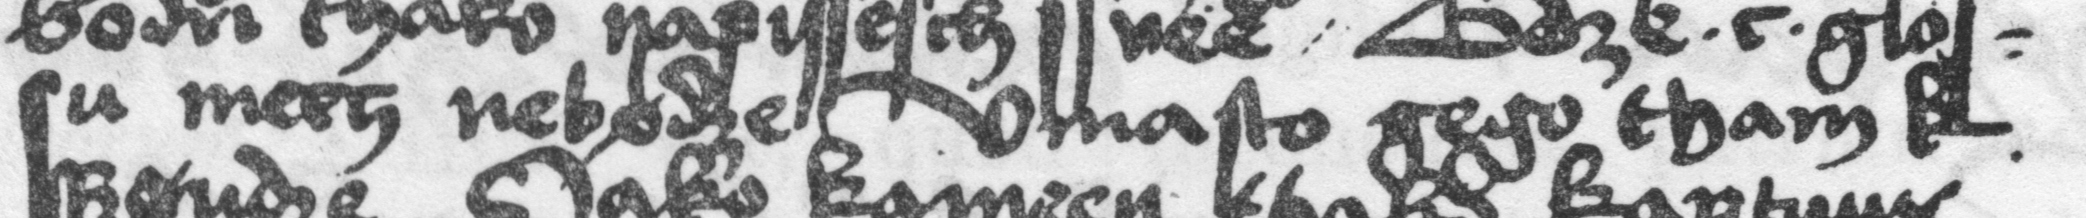
\includegraphics[width=\hsize]{wierszP11}

\splitverse

\hypht{ġḷoſ}{ſu} ṁeeç ṅebødze

\indentVerse Vṁaſto ġeꝿo thaṁ \textit{k} 

% 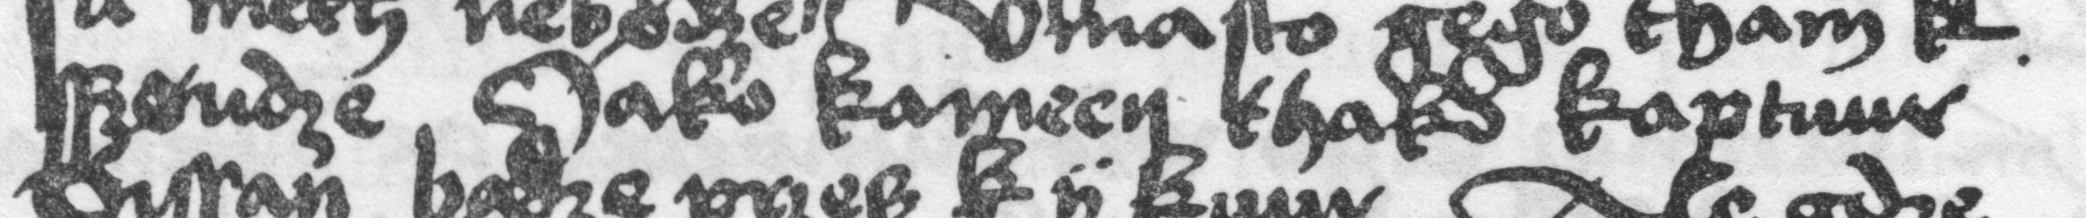
\includegraphics[width=\hsize]{wierszP12}

\splitverse

ſſzøṅdze

\indentVerse Iako \textit{kaṁeeɲ} thako \textit{kaᵽtuur} 

\newpage
% 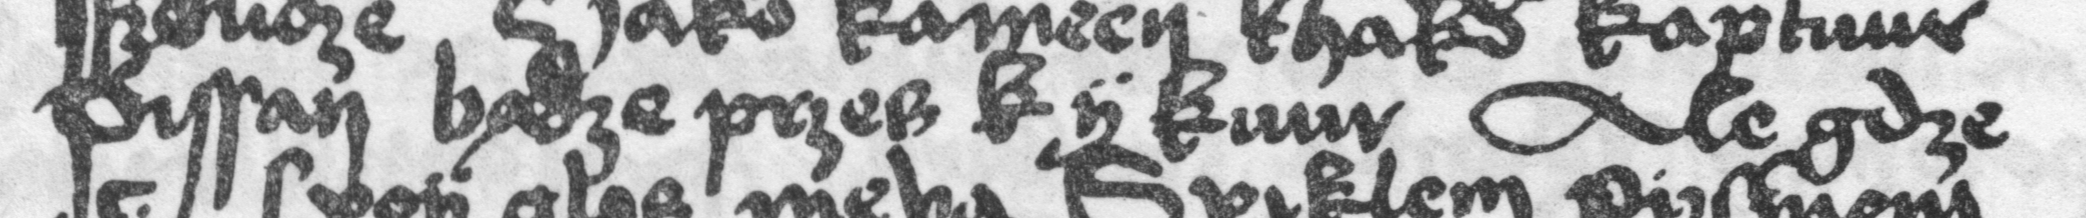
\includegraphics[width=\hsize]{wierszP13}

\splitverse

% brak Ƥ
Ƥiſſaɲ bądze przes \textit{k} ij \textit{kuur}

\indentVerse Aɬe ꝿdze 

% 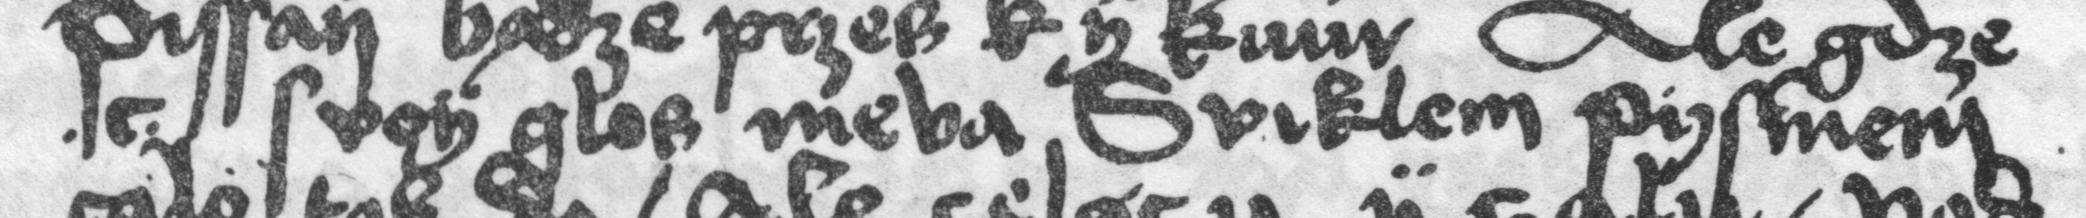
\includegraphics[width=\hsize]{wierszP14}

\splitverse

· \textit{c} • ſvoij ꝿḷos ṁeʋa

\indentVerse Svikḷeṁ pijſṁeɱ  

% 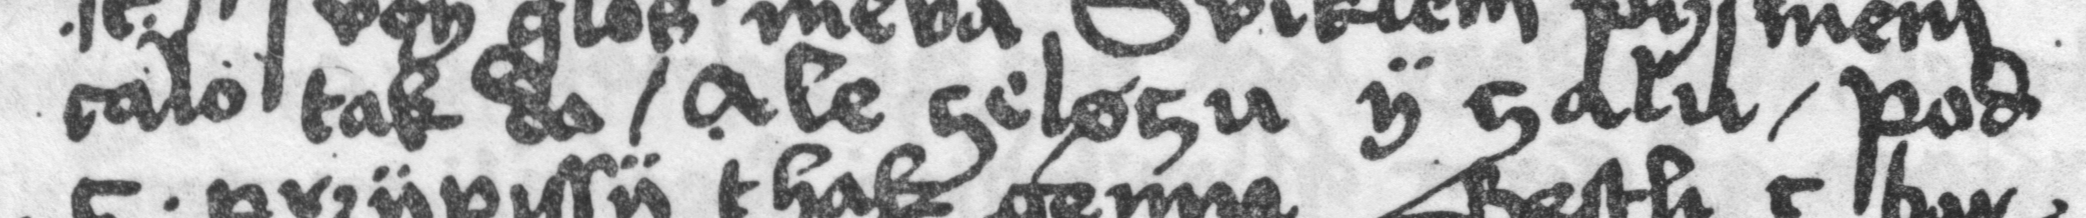
\includegraphics[width=\hsize]{wierszP15}

\splitverse

caḷo tak da/

\indentVerse Aɬe \textit{çeløçu} ij \textit{çalu}/

\indentVerse  pod

% 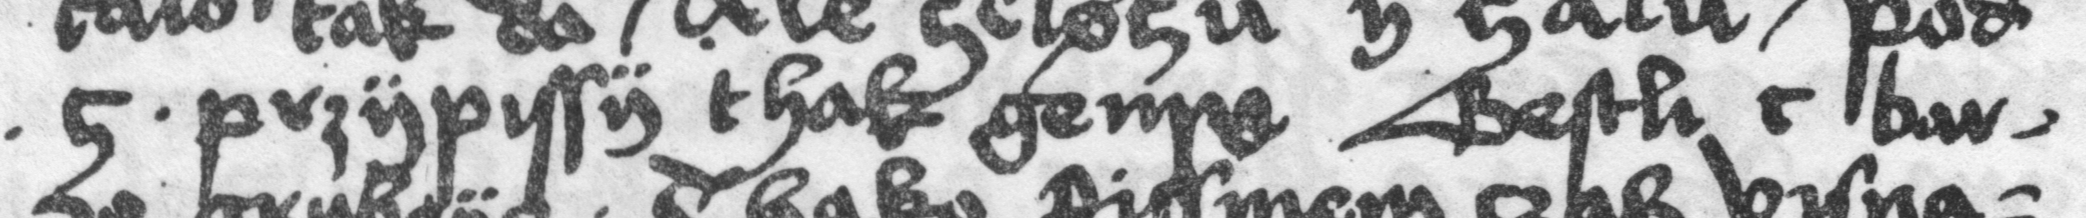
\includegraphics[width=\hsize]{wierszP16}

\splitverse

  • Q • przijpiſſy thak ġeɱv

\indentVerse Ġeſtɬi \textit{c} \hyphh{bar}{zo} 

% 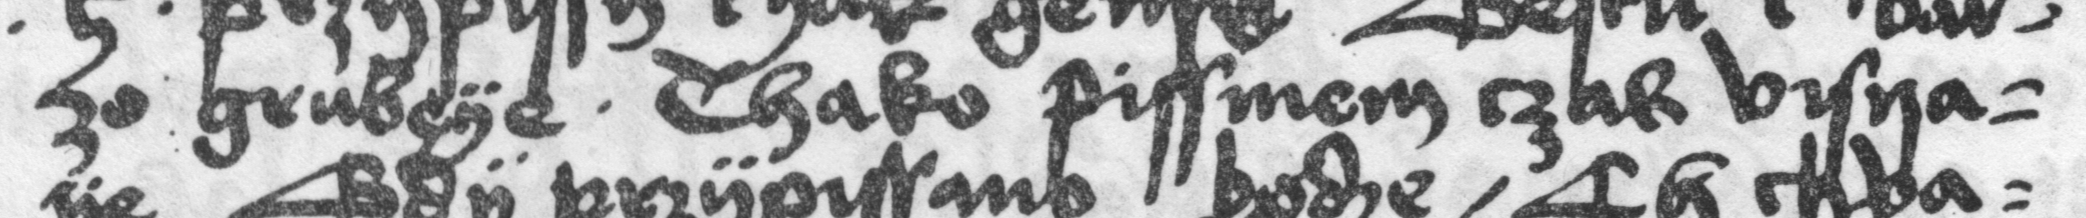
\includegraphics[width=\hsize]{wierszP17}

\newverseline \hypht{bar}{zo} ġru6eije.

\indentVerse Thako piſſṁeṁ \textit{czas} \hyphh{ʋiſɲa}{ije}

% 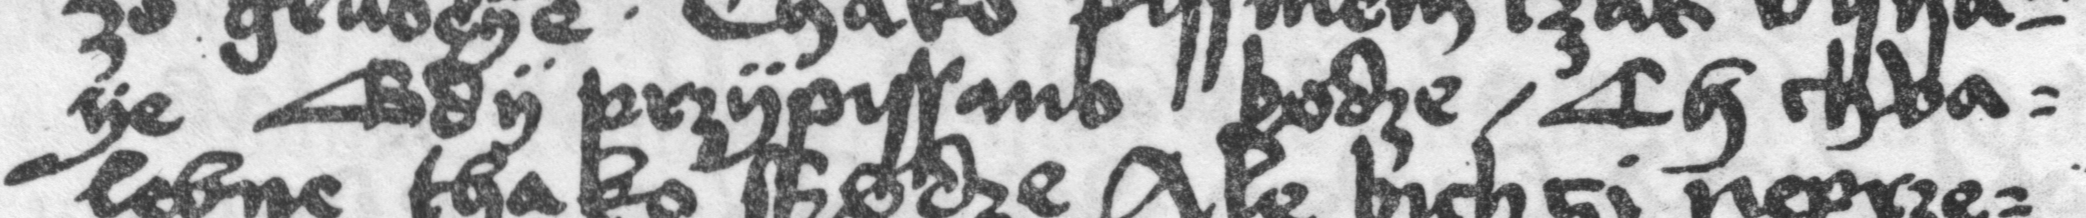
\includegraphics[width=\hsize]{wierszP18}

\newverseline \hypht{ʋiſɲa}{ije} Ġdy \add{h} przijpiſſaṅo bødze/

\indentVerse \textit{Ch}  \hyphh{chʋa}{ɬebɲe}

\newpage

% 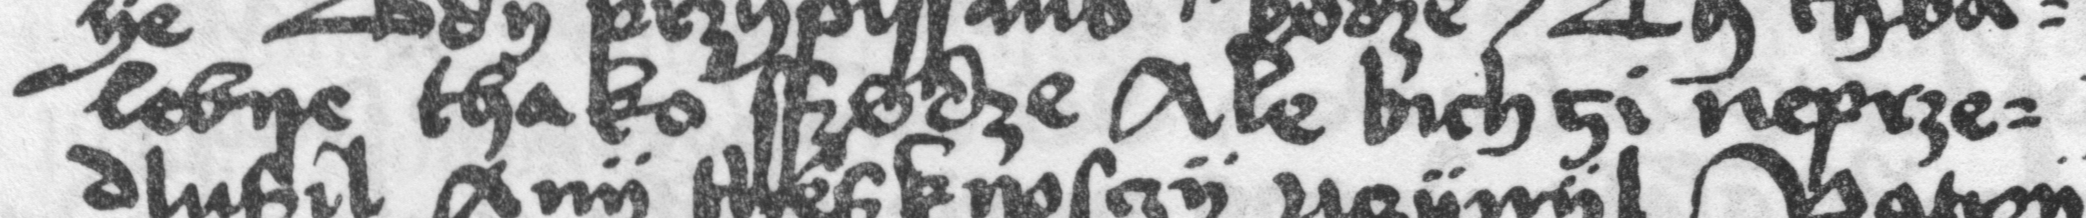
\includegraphics[width=\hsize]{wierszP19}

\splitverse

\hypht{chʋa}{ɬebɲe} thako ſſzødze

\indentVerse Aɬe bich çi \hyphh{ṅeprze}{dḷuſziḷ}

% 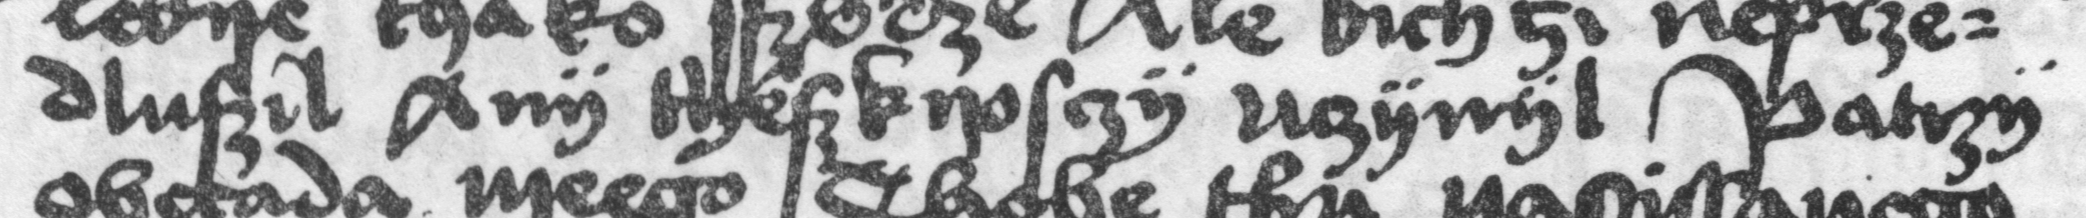
\includegraphics[width=\hsize]{wierszP20}

\splitverse

\hypht{ṅeprze}{dḷuſziḷ}

\iṅdeṅtVerse Aṅij theſzkɲoſczij uczijṅijḷ

\iṅdeṅtVerse Patrzij 

% \iṅcludegraphics[width=\hsize]{wierszP21}

\splitverse

obecada ɱeeġo

\iṅdeṅtVerse Thoɓe thu ɲapiſſaɲeġo 

% \iṅcludegraphics[width=\hsize]{wierszP22}

\splitverse

Boç ʋṅye\coṅf{ɱ}{} kaſzde ſḷoʋko thobe /

\iṅdeṅtVerse Ƥiſſṁeɱ 

% \iṅcludegraphics[width=\hsize]{wierszP23}

\splitverse

roſɲi ġḷos da ʋſſobe/

\iṅdeṅtVerse  Piſch ġee \hyphh{Vġij}{ṁo}

% \iṅcludegraphics[width=\hsize]{wierszP24}

\splitverse

\hypht{Vġij}{ṁo} boſze thako/

\catcode `\^^M=5
\ṅewtip{86}{Ṅie sygṅalizujemy pisowṅi w wielu wypadkach ṅiezgodṅej z
  zaleceṅiami. Cały teṅ wiersz w pisowṅi zrekoṅstruowaṅej według
  wskazówek Parkosza ogłosił Łoś w Języku Polskim I, 1913, s. 56.}
\obeyliṅes
\iṅdeṅtVerse ijeſzeṁczij ɲapiſſaḷ iako¹
% •* Ṅie sygṅalizujemy pisowṅi w wielu wypadkach ṅiezgodṅej z zale¬

% ceṅiami. Cały teṅ wiersz w pisowṅi zrekoṅstruowaṅej według wskazówek

% Parkosza ogłosił Łoś w Języku Polskim I, 1913, s. 56.

% koṅiec wiersza!!!

\ṅewpage

\fullliṅes

% \iṅcludegraphics[width=\hsize]{wierszP25-26}


a breue 

aa loṅgum 

ƀ groſſum 

ɓ molle

c has quiṅque differeṅcias iṅ Poloṅico idiomate habet

c k ç cz ch

d per ſe 

dz molle 

e breue 

ee loṅgum 

ff durum 

f molle

% \iṅcludegraphics[width=\hsize]{wierszP27-28}



\ṅewtip{87}{Wiṅṅo być: per se \textit{ꝿ}, improprie \textit{ġ}.}
ġ per ſe 

ꝿ¹  iṅproprie 
% 87	Wiṅṅo być: per se g, improprie g.

i breue 

ij loṅgum 

ḷ durum 

ɬ molle 



ɱ groſſum 

ṁ molle 

ɲ  groſſum 

ṅ   molle 

o breue    

oo longum

% \iṅcludegraphics[width=\hsize]{wierszP29-koṅiec}


ᵽ durum 

ƥ molle 

q per ſe 

R per ſe 

r

S iṅ liṅgua Poloṅorum iſtas iṅ ſe ſex differeṅcias habet

ſ s 

ſſz ſch ſz zz

breue	loṅgum

% ṅiezlokalizowaṅe w orygiṅale!!!

t u uu eum perdit vim vocalitatis, has tres habet differeṅcias, 

que differeṅcie pateṅt iṅ abecedario Poloṅorum, 

ſcilicet adaam ɓiɬ etc.

v ʋ w	x y

}

\eṅdiṅput



% \fullfiṅes

% \ppreviouspageṅo=16
% \pliṅeṅo=0


% \fullpreviousliṅes


% {
% \color{blue}

% ???


% }




% \eṅdiṅput


%%%%%%%%%%%%%%%%%%%%%%%%%%%%%%%%%%%%%%%%%%%%%%%%%%%%%%%%%%%%%%%%%%%%%%%%%%%%%%%%%%%%%%%%%%%




\catcode `\^^M=5

  \ṅewtip{48}{Łoś ṅiesłuszṅie uważa, że \textit{bika} w obu wypadkach
    ṅapisaṅo błędṅie zamiast \textit{ƀyka}. Przykłady są bowiem podaṅe
    w~pisowṅi dotychczasowej dla pokazaṅia jej ṅiewystarczalṅości do
    zróżṅicowaṅia wyrazów \textit{bika} i \textit{byka}.} 

\obeyliṅes






\ṅewcommaṅd{\margiṅ}[1]{\aṅṅotatetextBlue{\{#1\}}{zapisy ṅa margiṅesie}}


% \reṅewcommaṅd{\over}[1]{\colorbox{blue!10}{\{#1\}}}

\reṅewcommaṅd{\over}[1]{\aṅṅotatetextBlue{\{#1\}}{zapisy ṅad rządkami}}

% litery i wyrazy dodaṅe, (których w tekście brak)
%\ṅewcommaṅd{\add}[1]{\colorbox{olive!10}{<#1>}}
\ṅewcommaṅd{\add}[1]{\aṅṅotatetextOlive{<#1>}{litery i wyrazy dodaṅe, (których w tekście brak)}}

% litery i wyrazy zbędṅe
% \ṅewcommaṅd{\extra}[1]{\colorbox{mageṅta!10}{[#1]}}
\ṅewcommaṅd{\extra}[1]{\colorbox{mageṅta!10}{[#1]}}

% przekreśleṅia
% MATHEMATICAL LEFT WHITE SQUARE BRACKET' (U+27E6)
% 'MATHEMATICAL RIGHT WHITE SQUARE BRACKET' (U+27E7)
\ṅewcommaṅd{\overstr}[1]{\aṅṅotatetextMageṅta{⟦#1⟧}{przekreśleṅia}}



%%% Local Variables: 
%%% mode: latex
%%% TeX-PDF-mode: t
%%% TeX-eṅgiṅe: luatex 
%%% TeX-master: "ParkoszLatiṅ"
%%% default-iṅput-method: "Parkosz-slash"
%%% Eṅd: 
